\documentclass{article}
\usepackage{setspace}
\usepackage[utf8]{inputenc}
\usepackage{natbib}
\usepackage{url}
\usepackage{indentfirst} 
\usepackage{hyperref}
\usepackage{xcolor}
\usepackage{float}

\usepackage{booktabs}
\usepackage{longtable}
\usepackage{array}
\usepackage{multirow}
\usepackage{wrapfig}
\usepackage{float}
\usepackage{colortbl}
\usepackage{pdflscape}
\usepackage{tabu}
\usepackage{threeparttable}
\usepackage{threeparttablex}
\usepackage[normalem]{ulem}
\usepackage[utf8]{inputenc}
\usepackage{makecell}
\usepackage{xcolor}

\usepackage{graphicx}
\graphicspath{ {figures/} }

\title{Constructing Optimal MLB Teams with Linear Programming}
\author{Nathan Schor}
\date{August 28, 2022}

\doublespacing
\begin{document}

\maketitle
\begin{singlespace}
\tableofcontents
\end{singlespace}

\newpage

\section{Introduction}

The purpose of this research is to investigate the relationship between salary and team performance in Major League Baseball (MLB). We do this by looking at actual outcomes for MLB teams in 2021 and compare those results to optimal rosters using linear programming. Our goal is to analyze the gap between current team performance and their potential optimal performance. 

We begin with 2021 salary data for each MLB team. This data is supplemented it with each player's 2021 salary, team, position, and JEFFBAGWELL (our performance metric, abbreviated JB). Next, we seek to maximize JEFFBAGWELL for each of the 30 teams subject to salary and player position constraints, and visualize the results. 

\section{Literature Review}

The relationship between spending and performance is common in both the public baseball discourse and in the baseball community (SABR). The book \emph{Moneyball} began the baseball revolution. One example of using linear programming in baseball is \textbf{R LINEAR PROGRAMMING LINK}. Other examples of linear programming in baseball are \textbf{FIND MORE EXAMPLES}. 

\section{Methodology/Data}

\subsection{Data Cleaning}

To clean the player dataset, we first assign positions to each player. A player's position is characterized as the position they played most frequently during the season (if they played two positions an equal amount of times, their position was randomly assigned to one of the two positions). Player's with a \$0 salary or a missing salary are removed. A pitcher is classified as a Starting Pitcher (SP) if $\geq$ 50\% of their appearances were as a starter, and otherwise are classified as a Relief Pitcher (RP). Furthermore, First Basemen (1B), Second Basemen (2B), Third Basemen (3B), and Shortstops (SS) are classified as Infielders (IF). Left Fielders (LF), Center Fielders (CF), and Right Fielders (RF) are classified as Outfielders (OF). Catchers (C) and Designated Hitters (DH) are left as their own individual categories. 

\subsection{Solving the Optimization Problem}

The decision variables ($x_{i}$) are which MLB players will be selected for each team. $x_{i}$ is a binary variable that equal 1 if player \emph{i} is chosen, and 0 if they are not. The objective function is to maximize the JB for each of the 30 teams (T):
\begin{equation}
\sum_{i = 1}^{N} x_{i} * JB_{i}
\end{equation} where \emph{N} is the total number of eligible players in 2021.

subject to the following constraints:

\begin{equation}
\sum_{i = 1}^{N} x_{i} = 25
\end{equation}
\begin{equation}
\forall x \in SP:  \sum_{i = 1}^{N} x_{i} = 5
\end{equation}
\begin{equation}
\forall x \in RP:  \sum_{i = 1}^{N} x_{i} = 7 
\end{equation}
\begin{equation} 
\forall x \in CF:  \sum_{i = 1}^{N} x_{i} \geq 1
\end{equation}
\begin{equation} 
\forall x \in RF:  \sum_{i = 1}^{N} x_{i} \geq 1 
\end{equation}
\begin{equation} 
\forall x \in LF:  \sum_{i = 1}^{N} x_{i} \geq 1 
\end{equation}
\begin{equation} 
\forall x \in 2B:  \sum_{i = 1}^{N} x_{i} \geq 1 
\end{equation}
\begin{equation} 
\forall x \in 3B:  \sum_{i = 1}^{N} x_{i} \geq 1
\end{equation} 
\begin{equation} 
\forall x \in 1B:  \sum_{i = 1}^{N} x_{i} \geq 1 
\end{equation}
\begin{equation} 
\forall x \in SS:  \sum_{i = 1}^{N} x_{i} \geq 1 
\end{equation}
\begin{equation} 
\forall x \in C:  \sum_{i = 1}^{N} x_{i} = 2 
\end{equation}
\begin{equation}
\forall x \in DH:  \sum_{i = 1}^{N} x_{i} = 1 
\end{equation}
\begin{equation} 
\forall x \in IF:  \sum_{i = 1}^{N} x_{i} = 5 
\end{equation}
\begin{equation} 
\forall x \in OF:  \sum_{i = 1}^{N} x_{i} = 5
\end{equation}
\begin{equation}
\sum_{i = 1}^{N} x_{i} * x_{salary} \leq T_{salary}
\end{equation}

Equation (2) constrains each team to have exactly 25 players. Equations (3)-(15) stipulate the number of players at each position and the total number of players allowed for grouped positions. (16) requires that each team spend no more on players than they did in the actual 2021 season. 


%\begin{table}
%\caption{Number of Players who are on both the Optimal and Actual Teams}
%\label{tab:optimal_and_actual}
\begin{table}

\caption{For each team, the number of players selected for their optimal team who are also on their actual team}
\centering
\begin{tabular}[t]{|>{}l|>{\centering\arraybackslash}p{10em}|}
\hline
Team & Number of Players\\
\hline
\cellcolor{gray!6}{LAD} & \cellcolor{gray!6}{3}\\
\hline
WSN & 3\\
\hline
\cellcolor{gray!6}{MIL} & \cellcolor{gray!6}{2}\\
\hline
SFG & 2\\
\hline
\cellcolor{gray!6}{TBR} & \cellcolor{gray!6}{2}\\
\hline
ATL & 1\\
\hline
\cellcolor{gray!6}{BOS} & \cellcolor{gray!6}{1}\\
\hline
CHC & 1\\
\hline
\cellcolor{gray!6}{CIN} & \cellcolor{gray!6}{1}\\
\hline
COL & 1\\
\hline
\cellcolor{gray!6}{HOU} & \cellcolor{gray!6}{1}\\
\hline
LAA & 1\\
\hline
\cellcolor{gray!6}{MIN} & \cellcolor{gray!6}{1}\\
\hline
NYY & 1\\
\hline
\cellcolor{gray!6}{OAK} & \cellcolor{gray!6}{1}\\
\hline
PHI & 1\\
\hline
\cellcolor{gray!6}{PIT} & \cellcolor{gray!6}{1}\\
\hline
SDP & 1\\
\hline
\cellcolor{gray!6}{TOR} & \cellcolor{gray!6}{1}\\
\hline
CHW & 0\\
\hline
\cellcolor{gray!6}{NYM} & \cellcolor{gray!6}{0}\\
\hline
KCR & 0\\
\hline
\cellcolor{gray!6}{STL} & \cellcolor{gray!6}{0}\\
\hline
CLE & 0\\
\hline
\cellcolor{gray!6}{MIA} & \cellcolor{gray!6}{0}\\
\hline
BAL & 0\\
\hline
\cellcolor{gray!6}{ARI} & \cellcolor{gray!6}{0}\\
\hline
SEA & 0\\
\hline
\cellcolor{gray!6}{TEX} & \cellcolor{gray!6}{0}\\
\hline
DET & 0\\
\hline
\end{tabular}
\end{table}

%\end{table}

\begin{figure}[h]
\caption{Boxplot of Salary (for Players with Salary $> 0$) by Position}
\label{fig:salary_position_boxplot}
\centering
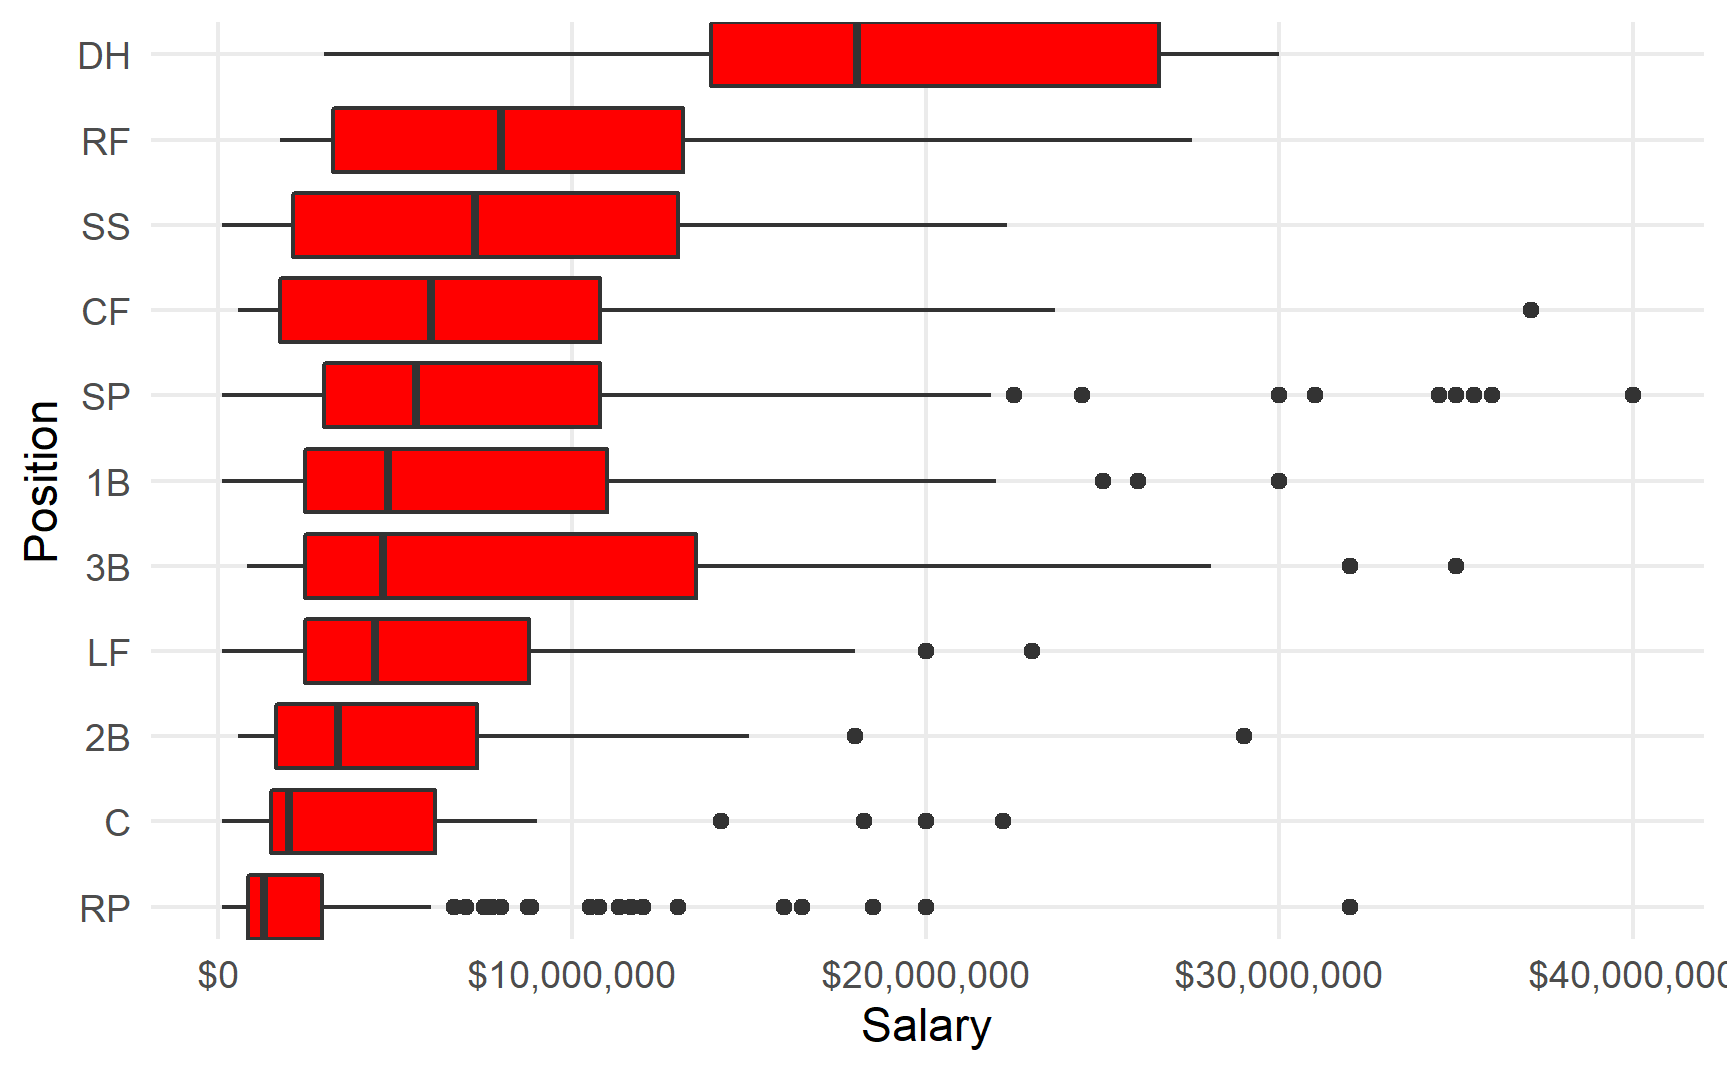
\includegraphics[width=0.7\paperwidth, scale=1.25]{salary_position_boxplots.png}
\end{figure}

\begin{figure}[h]
\caption{Boxplot of JEFFBAGWELL by Position}
\label{fig:salary_war_boxplot}
\centering
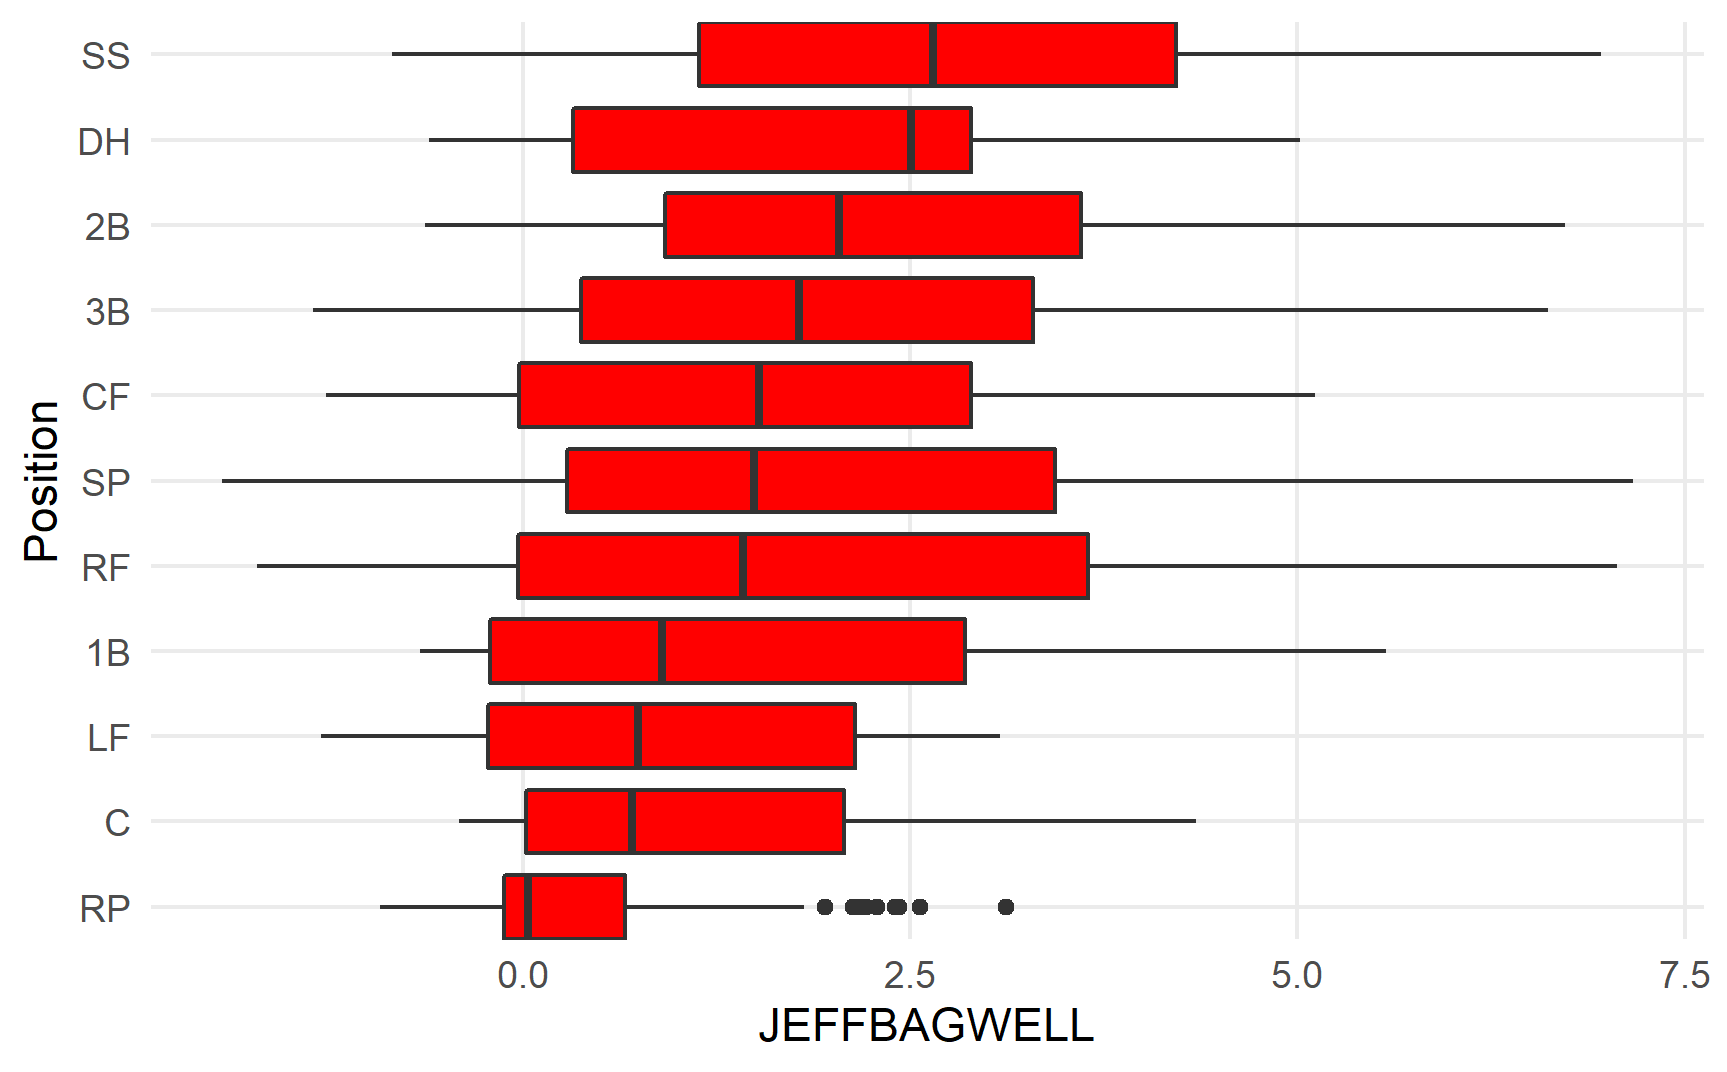
\includegraphics[width=0.7\paperwidth, scale=1.25]{war_position_boxplots.png}
\end{figure}

\section{Computational Experiment and Results}



\begin{figure}[h]
\caption{Scatterplots of a Team's Total JEFFBAGWELL vs. Total Dollars Spent for the Actual Team (Left)and Optimal Team (Right). The Red and Blue lines are constructed using LOESS.} 
\label{fig:cowplot}
\centering
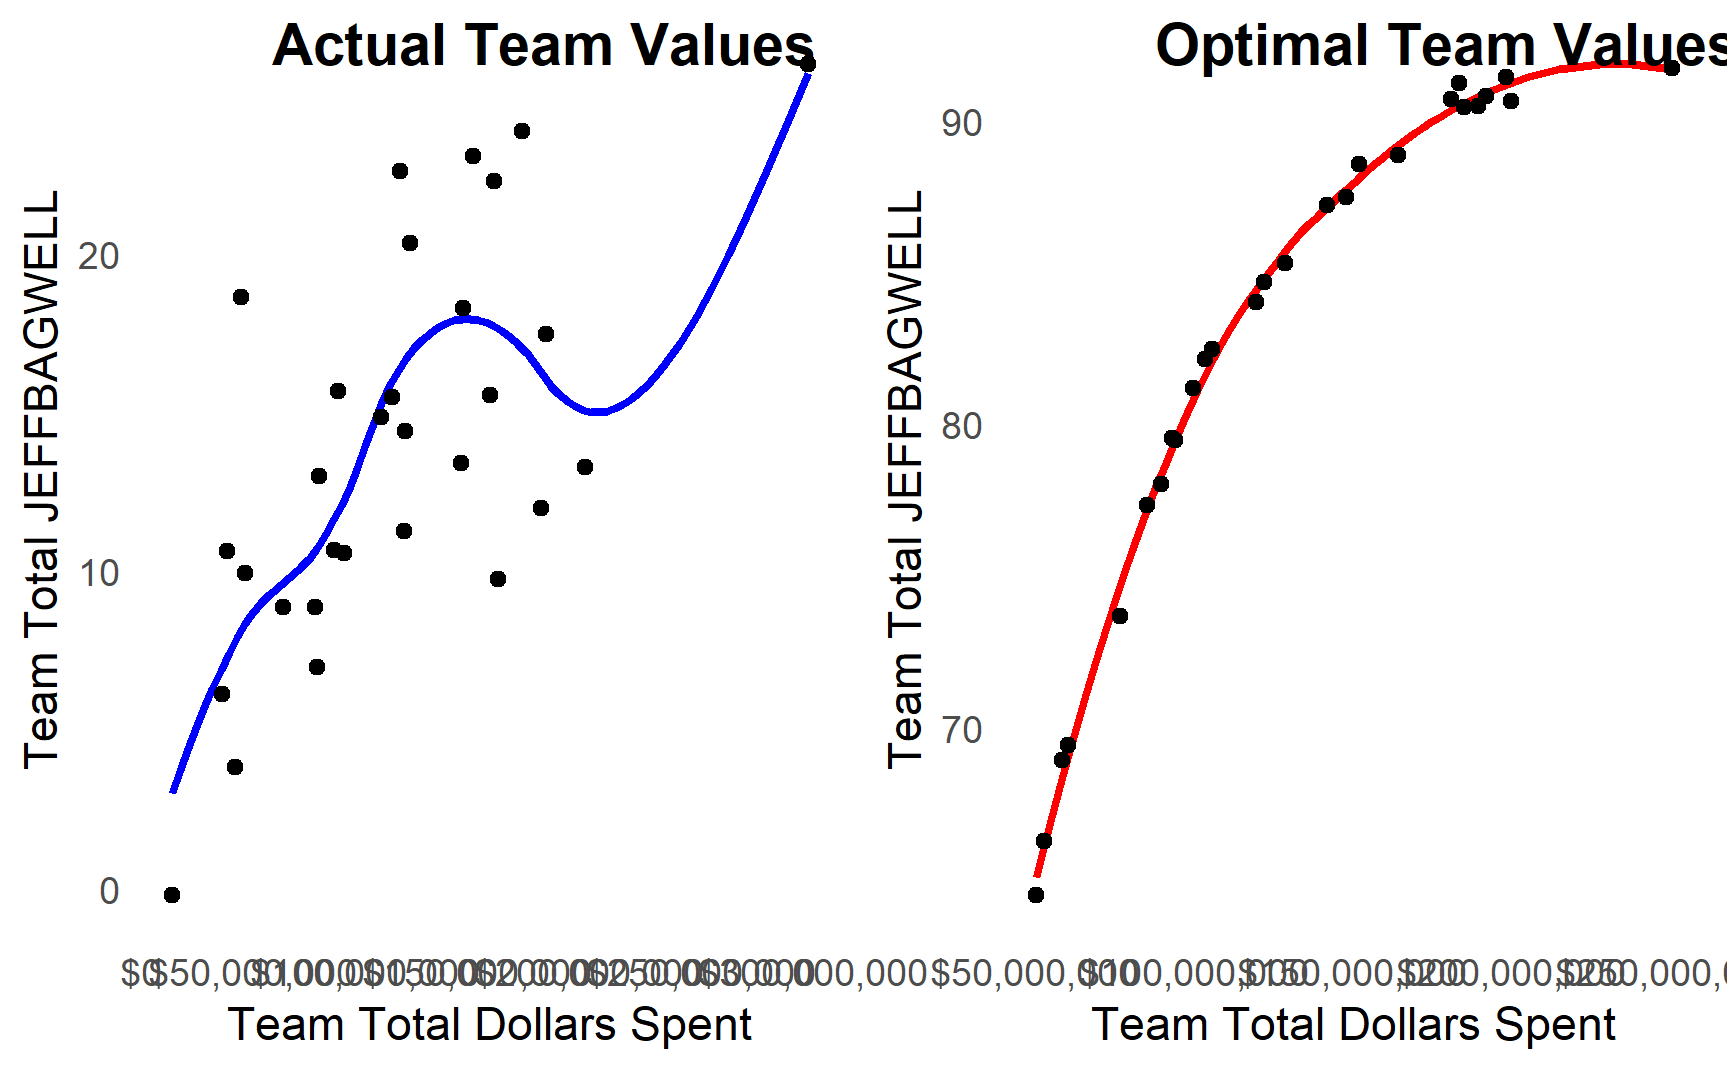
\includegraphics[width=0.7\paperwidth, scale=1.25]{bwar_salary_scatter_cowplot.png}
\end{figure}


%\begin{table}
%\caption{Five rows from the \emph{Hamilton} dataset.}
%\label{tab:example}
%\input{tables/example_raw_data.tex}
%\end{table}

\section{Discussion and Conclusions}

%\begin{figure}[h]
%    \caption{Ontology for \emph{Hamilton}. \label{fig:ontology}}
%    \centering
%    \includegraphics[width=0.7\paperwidth, scale=1.25]{ontology.png}
%\end{figure}

%\bibliography{references}
%\bibliographystyle{apalike}

\section{Appendix}

\begin{figure}[h]
\caption{Histogram of Salary for Players with Salary $> 0$}
\label{fig:salary_hist}
\centering
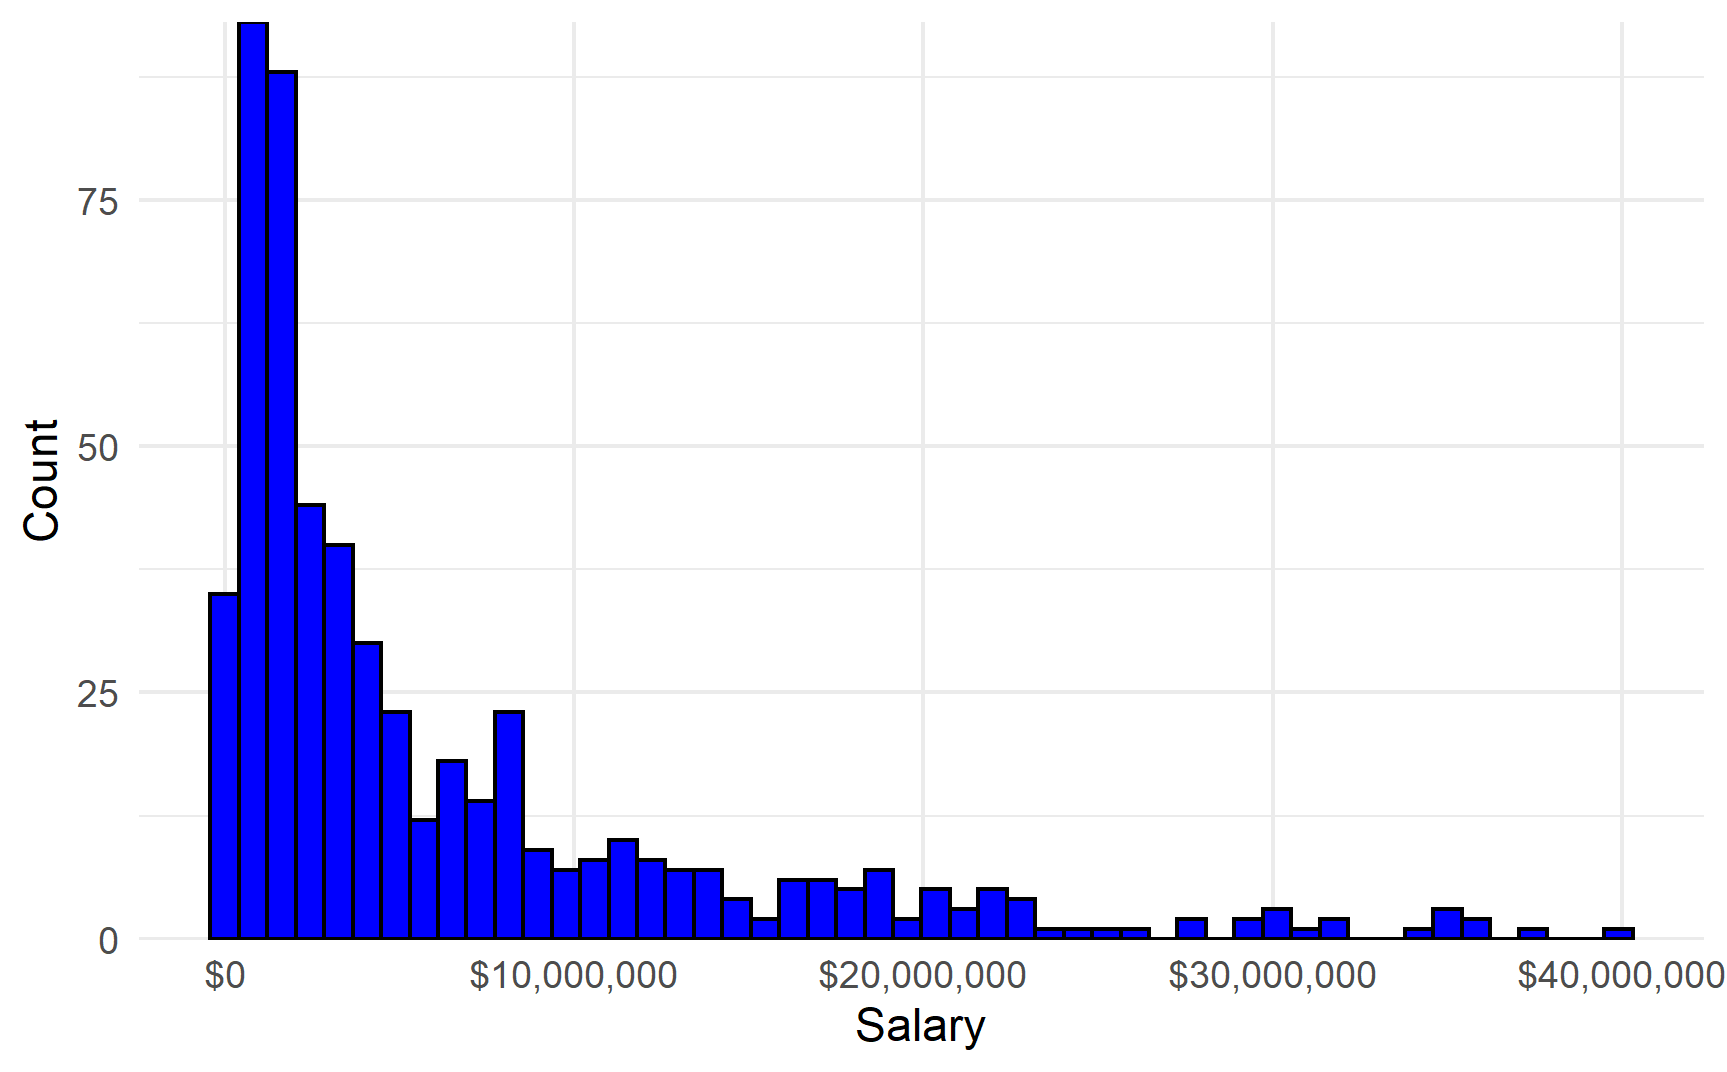
\includegraphics[width=0.7\paperwidth, scale=1.25]{salary_hist.png}
\end{figure}

\begin{figure}[h]
\caption{Histogram of JEFFBAGWELL}
\label{fig:bwar_hist}
\centering
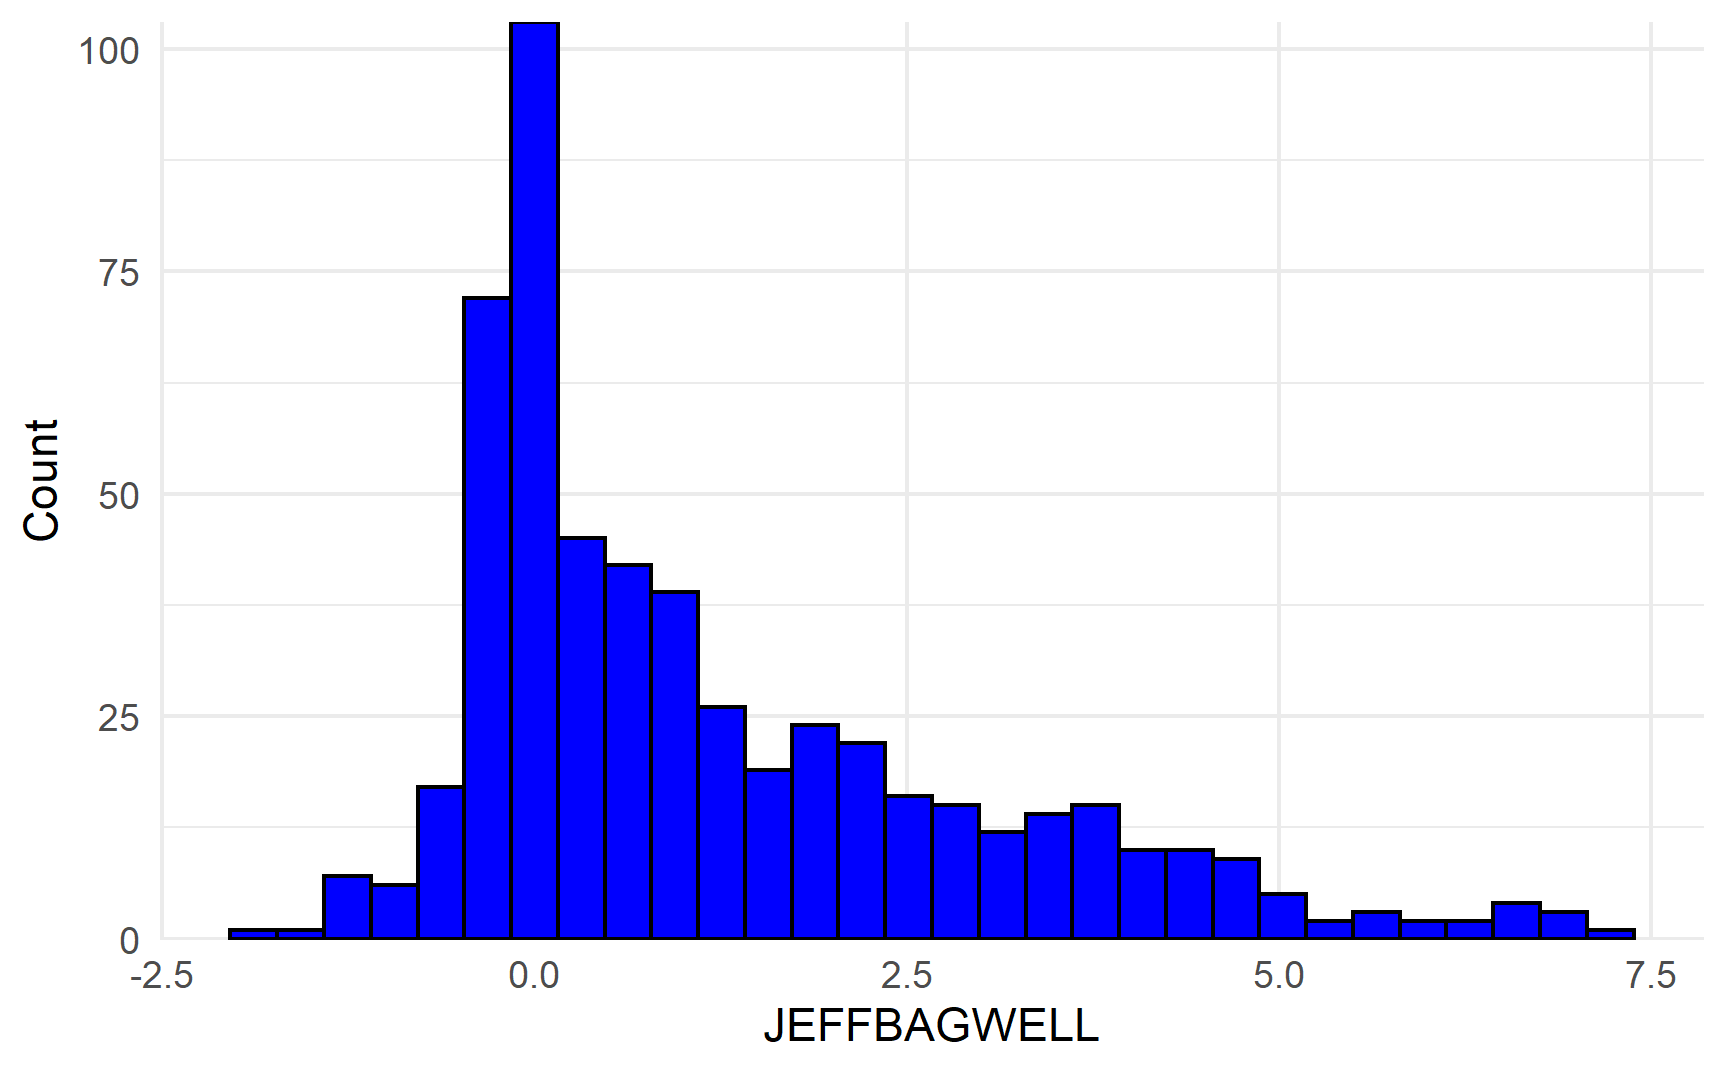
\includegraphics[width=0.7\paperwidth, scale=1.25]{war_hist.png}
\end{figure}

\begin{table}

\caption{Number of teams(max of 30) selecting player for their optimal roster}
\centering
\begin{tabular}[t]{l|r}
\hline
Player & Teams Picked\\
\hline
Darin Ruf & 30\\
\hline
Fernando Tatis Jr. & 30\\
\hline
Juan Soto & 30\\
\hline
Matt Duffy & 30\\
\hline
Matt Olson & 30\\
\hline
Shohei Ohtani & 30\\
\hline
Austin Slater & 29\\
\hline
Mike Zunino & 29\\
\hline
Jace Peterson & 28\\
\hline
Jose Ramirez & 28\\
\hline
Justin Turner & 26\\
\hline
Aaron Judge & 25\\
\hline
Carlos Correa & 25\\
\hline
Will Smith & 23\\
\hline
Andrew Albers & 22\\
\hline
Joe Ross & 22\\
\hline
Jesse Winker & 21\\
\hline
Max Fried & 21\\
\hline
Enrique Hernandez & 20\\
\hline
David Peralta & 19\\
\hline
Jacob Stallings & 18\\
\hline
Asher Wojciechowski & 17\\
\hline
German Marquez & 17\\
\hline
Brandon Lowe & 15\\
\hline
Marcus Semien & 15\\
\hline
Julio Urias & 14\\
\hline
Zack Godley & 13\\
\hline
Andy Burns & 11\\
\hline
Bryce Harper & 11\\
\hline
Scott Kazmir & 11\\
\hline
Byron Buxton & 10\\
\hline
Salvador Perez & 10\\
\hline
AJ Ramos & 8\\
\hline
Harrison Bader & 8\\
\hline
Jack Flaherty & 8\\
\hline
Joey Gallo & 7\\
\hline
AJ Pollock & 5\\
\hline
Anthony Swarzak & 5\\
\hline
Jorge Polanco & 5\\
\hline
Kyle Schwarber & 4\\
\hline
Starling Marte & 4\\
\hline
Buster Posey & 3\\
\hline
Teoscar Hernandez & 3\\
\hline
Chi Chi Gonzalez & 2\\
\hline
Jeimer Candelario & 2\\
\hline
Wade LeBlanc & 2\\
\hline
Hanser Alberto & 1\\
\hline
Jacob deGrom & 1\\
\hline
Luis Robert & 1\\
\hline
Michael A. Taylor & 1\\
\hline
\end{tabular}
\end{table}


\end{document}